\documentclass[
	%parspace, % Térköz bekezdések közé / Add vertical space between paragraphs
	%noindent, % Bekezdésének első sora ne legyen behúzva / No indentation of first lines in each paragraph
	%nohyp, % Szavak sorvégi elválasztásának tiltása / No hyphenation of words
	%twoside, % Kétoldalas nyomtatás / Double sided format
	%draft, % Gyorsabb fordítás ábrák rajzolása nélkül / Quicker draft compilation without rendering images
	%final, % Teendők elrejtése / Set final to hide todos
]{elteikthesis}[2020/11/23]
\usepackage{glossaries}
\usepackage{hyperref}
\makeglossaries

% Dolgozat metaadatai
% Document's metadata
\title{Network resource management in Kubernetes} % cím / title
\date{2021} % védés éve / year of defense

% Szerző metaadatai
% Author's metadata
\author{Kristóf Aranyos}
\degree{Computer Science BSc}

% Témavezető(k) metaadatai
% Superivsor(s)' metadata
\supervisor{Ferenc Fejes} % belső témavezető neve / internal supervisor's name
\affiliation{PhD Candidate} % belső témavezető beosztása / internal supervisor's affiliation
%\extsupervisor{Külső Kornél} % külső témavezető neve / external supervisor's name
%\extaffiliation{informatikai igazgató} % külső témavezető beosztása / external supervisor's affiliation

% Egyetem metaadatai
% University's metadata
\university{Eötvös Loránd University}
\faculty{Faculty of Informatics}
\department{Institute of Computer Science\\Department of Information Systems}
\city{Budapest} % város / city
\logo{elte_cimer_szines} % logo

% Irodalomjegyzék hozzáadása
% Add bibliography file
\addbibresource{thesis.bib}

% A dolgozat
% The document
\begin{document}

% Nyelv kiválasztása
% Set document language
\documentlang{english}
%\documentlang{english}

% Teendők listája (final dokumentumban nincs)
% List of todos (not in the final document)
%\listoftodos[\todolabel]

% Dokumentum beállítások
% Some document settings
% Lábjegyzet folytonos számozása fejezetek között
% Continuous counting of footnotes among chapters
\counterwithout{footnote}{chapter}

% Tartalomjegyzék oldalszámozásának rejtése
% Hide page numbering of ToC
\newcounter{conpageno}
\let\oldtableofcontents\tableofcontents
\renewcommand{\tableofcontents}{
	\pagenumbering{gobble}
	\oldtableofcontents
	\cleardoublepage
	\setcounter{conpageno}{\value{page}}
	\pagenumbering{arabic}
	\setcounter{page}{\value{conpageno}}
}


% Címlap (kötelező)
% Title page (mandatory)
\maketitle
\topicdeclaration


% Tartalomjegyzék (kötelező)
% Table of contents (mandatory)
\tableofcontents
\cleardoublepage

\newglossaryentry{api}
{
    name=API,
    description={Acronym for Application Programming Interface, a system that lets two applications communicate}
}

\newglossaryentry{on-premises}
{
    name=on-premises,
    description={A setup where software runs on the own machines of a user or organization, instead of cloud providers}
}

\newglossaryentry{ml}
{
    name=ML,
    description={Acronym for machine learning, which is a branch of computer science}
}

\newglossaryentry{cri}
{
    name=CRI,
    description={Acronym for Container Runtime Interface, an unified interface for container runtimes}
}

\newglossaryentry{load-balancer}
{
    name=load balancer,
    description={Distributes requests between given machines. This is used to scale the capacity of a system}
}

\newglossaryentry{ssl}
{
    name=SSL,
    description={Acronym for Secure Sockets Layer, or more properly, TLS (Transport Layer Security). A set of technologies allowing channels to be encrypted, preventing man-in-the-middle attacks}
}

\newglossaryentry{tuple}
{
    name=tuple,
    description={A finite ordered list. A tuple of n elements is called n-tuple}
}

\newglossaryentry{risc}
{
    name=RISC,
    description={Acronym for Reduced Instruction Set Computing which refers to an instruction set architecture that uses relatively few instructions}
}

\newglossaryentry{read-only}
{
    name=read-only,
    description={A register or memory location that can't be written to, only read from}
}

\newglossaryentry{fp}
{
    name=FP,
    description={Acronym for frame pointer. A highly specialized type of CPU register used for managing function calls}
}

\newglossaryentry{pc}
{
    name=PC,
    description={Acronym for program counter. A specialized CPU register that points to the next instruction to be executed}
}

\newglossaryentry{stack}
{
    name=stack,
    description={A general-purpose register that holds information about the call stack, which describes subroutine call order.}
}

\newglossaryentry{verifier}
{
    name=verifier,
    description={The eBPF verified is used to inspect the code before loading it into the kernel, making sure it doesn't contain unsafe code that can harm the system}
}

\newglossaryentry{kprobe}
{
    name=kprobe,
    description={Hooks that allow to run eBPF code when specific kernel functions are called}
}

\newglossaryentry{uprobe}
{
    name=uprobe,
    description={Hooks that allow to run eBPF code when specific user space functions are called}
}

\newglossaryentry{socket-buffer}
{
    name=socket buffer,
    description={A structure to hold data from a packet. It enables easy access and modification from code}
}

\newglossaryentry{tc}
{
    name=TC,
    description={Acronym for Traffic Control, an user space program used for configuring the Linux packet scheduler}
}

\newglossaryentry{edt}
{
    name=EDT,
    description={Acronym for Earliest Departure Time, an algorithm to limit the bandwidth of a given data stream by delaying packets}
}

\newglossaryentry{cpu}
{
    name=CPU,
    description={Acronym for Central Processing Unit, referring to the processor of a machine}
}

\newglossaryentry{ram}
{
    name=RAM,
    description={Acronym for Random Access Memory, used to store all temporary data in a machine}
}

\newglossaryentry{tree}
{
    name=tree,
    description={A hierarchical data structure made up from nodes ordered in layers. Each node can have multiple children but only one parent}
}

\newglossaryentry{ingress}
{
    name=ingress,
    description={An network interface where transmitted data enters a machine or process}
}

\newglossaryentry{egress}
{
    name=egress,
    description={A network interface where data exits a machine or process and gets transmitted}
}

\newglossaryentry{tbf}
{
    name=TBF,
    description={Acronym for Token Bucket Filter, which is an algorithm to limit bandwidth of a data stream. This is achieved by dropping non-conformant packets}
}

\newglossaryentry{latency}
{
    name=latency,
    description={The delay between two hosts on a network}
}

\newglossaryentry{tcp}
{
    name=TCP,
    description={Acronym for Transmission Control Protocol, which is a reliable protocol for data transmission, but slower than UDP}
}

\newglossaryentry{udp}
{
    name=UDP,
    description={Acronym for User Datagram Protocol, an unreliable but fast protocol for data exchange}
}

\newglossaryentry{netcode}
{
    name=netcode,
    description={A part of an application that deals with the data exchange over a network. It has to ensure data is reliably and correctly transmitted}
}

\newglossaryentry{transport-layer}
{
    name=transport layer,
    description={A conceptual layer in the network stack of the OSI model. Protocols in this layer deal with host-to-host communication and data multiplexing between processes}
}

\newglossaryentry{compiled}
{
    name=compiled,
    description={A type of programming language that requires the source code to be translated to machine-readable code before execution}
}

\newglossaryentry{statically-typed}
{
    name=statically typed,
    description={A type of language where the type of a variable is known at compile-time}
}

\newglossaryentry{garbage-collector}
{
    name=garbage collector,
    description={A programming language feature that automatically cleans up unused variables on the heap}
}

\newglossaryentry{memory-safe}
{
    name=memory-safe,
    description={A type of language with safety measures that prevent various memory-related errors such as buffer overflows, out-of-bounds writes and the like}
}

\newglossaryentry{oop}
{
    name=OOP,
    description={Acronym for Object Oriented Programming, a popular paradigm built around the concept of data hiding - also called encapsulation}
}

\newglossaryentry{ide}
{
    name=IDE,
    description={Acronym for Integrated Development Environment, software with built-in features to support development}
}

\newglossaryentry{float}
{
    name=floating-point numbers,
    description={A rational number stored as exponent and mantissa}
}

\newglossaryentry{rng}
{
    name=PRNG,
    description={Acronym for pseudo random number generator, an algorithm that outputs numbers that are seemingly - but not really random. The randomness depends on the seed used to initialzie the generator}
}

\newglossaryentry{mock}
{
    name=mock,
    description={A program object that pretends to behave like another one but has bare-bones implementation. Used for testing}
}

% Tartalom
% Main content
\chapter{Introduction} % Introduction
\label{ch:intro}

\section{Motivation}
I'm using Kubernetes\cite{kubernetes} daily at work. It's an excellent orchestration engine combined with an ecosystem that is both mature and diverse, but there are certain areas that still require further development. But what is Kubernetes?

Most services available on the world wide web today are running on some kind of autonomously scalable container orchestration system. One of the most widely used engines is Kubernetes, opted for by several industry leaders.

Kubernetes itself doesn't include networking, offloading this task to CNIs (Container Network Infrastructure). There are several of these freely available (such as Calico, Cilium, Flannel, WeaweNet, etc) but the feature set of these is wildly varying and their configuration is inconsistent. One of their deficiencies is that they don't support introducing bottlenecks in the network in order to test the quality of the services in, for example, a low-bandwidth or high-congestion networking environment.


\section{Results}
The goal of the thesis is to develop an application capable of simulating these conditions on Pod or Service level. The application is connected to the Kubernetes API, listening to Pod create, update and delete events. The Pods' containers get attached an EBPF program according to their metadata. These EBPF programs then run in kernel space and allow or drop packets to limit bandwidth and simulate network congestion.

To prove the effectiveness and correctness of the application, it will be benchmarked on various different systems and with multiple tools.

\section{Structure}
The thesis will consist of three main parts; User Guide, Developer Documentation, and Benchmarks.
\bigbreak

The User Guide will describe the general ideas behind the application as well as the system requirements, the installation guide, how to configure the limits for the system, and how to run the application.
\bigbreak

The Developer Documentation will contain a detailed description of the Kubernetes ecosystem, the Linux and EBPF ecosystem, and the details of the application's inner working. This latter will include a description of the implemented filters as well.
\bigbreak

The Benchmarks chapter will include findings on the performance of the application.
\cleardoublepage

\chapter{User Documentation} % User guide
\label{ch:user}

The User Documentation contains a basic overview of the application, the system requirements, an installation guide and instructions on how to use the application.

\section{System requirements}
\subsection{Hardware requirements}
The application itself is lightweight and doesn't require strong hardware. It however requires a Kubernetes cluster to work on, therefore Kubernetes' system requirements apply to it. It's worth to note, that serving tens of thousands if not more users (which Kubernetes clusters are intended for) needs multiple strong server machines. For testing purposes, a single pc or laptop will suffice. \\

There are two kind of Kubernetes nodes: Master and Worker nodes. In every cluster, there is one Master node, which controls the Workers. There is no limit on Worker count. It's possible to run a Master and a Worker node on one computer to avoid needing multiple machines.
\bigbreak

\newpage
\noindent
Hardware requirements of Kubernetes Master nodes:
\begin{itemize}
	\item CPU: At least two cores @ 1 GHz. X86-64 recommended, ARM64 might work, but it's untested. 
	\item RAM: At least 2 GB of free memory.
	\item Disk space: At least 2 GB recommended for the tooling (k8s-core, cert-updater, fluentd, kube-addon-manager, rescheduler, network, etcd, proxy, kubelet).
\end{itemize}

\noindent
Hardware requirements of Kubernetes Worker nodes:
\begin{itemize}
	\item CPU: At least one core @ 1 GHz. X86-64 recommended, ARM64 might work, but it's untested. 
	\item RAM: At least 700 Mb of free memory.
	\item Disk space: At least 1 GB recommended for the tooling (fluentd, dns, proxy, network, kubelet).
\end{itemize}

\newpage
\subsection{Software requirements}
While Kubernetes runs on Windows as well as on Linux, generally most servers will run the latter, and a core part of the application - the EBPF programs - also run in the Linux kernel. Therefore, Linux is required and while the code might compile on Windows or macOS, it certainly won't run on them.\\
Another thing worth mentioning is that EBPF requires a fairly new kernel to run as it's a bleeding edge technology. The development took place on a computer running Manjaro 20.1.1 with Linux 5.10.15 kernel.
\bigbreak

\noindent
Software requirements of the application:
\begin{itemize}
	\item Linux with kernel\cite{linux-kernel} 5.10 or newer
	\item Kubernetes\cite{kubernetes} v1.20 or newer, K3S\cite{k3s} is recommended for \underline{\gls{on-premises}} clusters
	\item Clang\cite{clang} 10.0 or newer
	\item BPF tools\cite{bpf-1}
	\item LibBPF\cite{libbpf}
	\item Go\cite{go} 1.15 or newer
\end{itemize}

\newpage
\section{Overview}
\begin{figure}[H]
	\centering
	
\includegraphics[width=\textwidth]{images/archi.png}
	\caption{Application architecture}
	\label{fig:app-arch}
\end{figure}
Simply put, the application manages the traffic flowing through a Kubernetes cluster according to a set of rules. These rules can be as simple as applying a bandwidth limit, or dropping given packets. They can also be much more complex through user defined programs, if required.
\bigbreak

The center of operation is an executable written in Golang that uses the Kubernetes API to constantly monitor the state of the cluster. On startup, it fetches all Kubernetes services and pods, reading their metadata to decide if a limit should be set on them. All limits are applied on the pods themselves, even service ones. Services are linked to a set of pods, their limits are inherited by the pods, though if a pod has colliding limit, the pod-level one is applied.
\bigbreak

Since a pod is not one process, but an abstraction above closely related ones, it's not possible to simply control their traffic. Instead, even though they are treated as one unit, the underlying processes are iterated and all of them are set to the same limits.
\bigbreak

\noindent
The process of applying limits is the following:
\texttt{
\begin{enumerate}
	\item Finding the pod on which the limit gets applied
	\item Iterate over the processes of the pod
	\begin{enumerate}
    	\item Get the cgroup of the process
    	\item\label{limitprocess:compiling} Compile a custom-tailored EBPF program using pre-written templates
    	\item Load the EBPF program into the Linux kernel
    	\item Attach the EBPF program the the cgroups' socket buffer hooks
    \end{enumerate}
	\item Save the limit info of the pod
\end{enumerate}
}
\noindent
[\ref{limitprocess:compiling}] The reason each pod is required to compile its own EBPF program is due to an inherent property of the EBPF system: it doesn't support parametrizing the programs. This is bypassed by the application using C macros that are set compile-time; further info about this in the Developer Documentation part.

\newpage
\section{Installation guide}
For development, Manjaro 20.1.1 with Linux 5.10.15 kernel was used. The Installation Guide will also be based on this.

\subsection{Initial setup}
\subsubsection{Linux kernel version}
The first step is to ensure a new enough linux kernel is running on the machine. The features used in the EBPF programs require a kernel version newer than 5.10. To check, open a terminal and run
\begin{verbatim}
$ uname -r 
\end{verbatim}
This outputs the version of the currently running kernel. If the kernel version is too old, a simple way to update it is to use the Manjaro Settings Manager. After opening it, click on Kernel. It will show a list of kernels available to be installed. Choose a version of 5.10 or over. Click install, then restart the machine and check the version again.

\subsubsection{Required software}
If the kernel is up to date, the next step is to install the required tools that will be used to compile the Go application, the EBPF programs - which, by the way are written in a subset of C - and load them into the kernel. The easiest way is to open a terminal and run
\begin{verbatim}
$ sudo pacman -S base-devel go clang bpf libbpf
\end{verbatim}
\noindent
This will install every required piece of software, namely:
\begin{enumerate}
    \item base-devel: This is a basic bundle of software that is used by virtually everything else.
    \item go: The Golang compiler and tooling. Required for compiling the application itself.
    \item clang: A C compiler used to generate the object files from C source code.
    \item bpf, libbpf: These utilities are used to load the object files into the kernel.
\end{enumerate}


\subsection{Kubernetes Cluster}
Kubernetes - being a complex software bundle - requires the help of guides to install. Since it's a core requirement, a short one is included in the thesis.\\
The project uses K3S due to the ease of setup, as it bundles a CNI (Flannel) and Ingress controller (Traefik). These require little to no configuration - something that's a severe problem when using raw kubeadm, kubelet and kubectl utilities.

\subsubsection{Using the bundled executable}
The easiest way to set up the cluster is to simply run the bundled executable. This is located in the  \textit{k3s} folder. Normally, including executables is to be avoided; in this case, the main motivations were a simple setup procedure and the fact that at the time of writing the application, the latest K3S releases weren't capable of using Cgroup v2. The fix was already done, a release had yet to be published.

\noindent
To start the Kubernetes cluster, open a terminal and run
\begin{verbatim}
$ sudo k3s/run.sh
\end{verbatim}

\noindent
This will start the master node with an additional worker node. The ramp-up period depends on the speed of the machine, generally, half a minute should be enough for it.

\subsubsection{Installing natively}
A more elaborate and recommended way to install the Kubernetes cluster is to follow the official way. This will set up a service on the machine that will by default start up on boot. This spares the burden of having to manually start the executable each time. To install the K3S service, open a terminal and run
\begin{verbatim}
$ curl -sfL https://get.k3s.io | sh -
\end{verbatim}

\noindent
The install script will automatically set up everything required to run the service, this usually takes around a minute or so. After installation, the cluster will automatically start to run, creating a master and a worker node. Ensure the service is running using
\begin{verbatim}
$ systemctl status k3s.service
\end{verbatim}

\subsubsection{Configuring the cluster}
Configuring the cluster itself is depenent on intent. For development or production clusters, this part can be skipped entirely as it follows the configuration of the example bundled service. \\

The example service is kept as minimal as possible to keep complexity down. The server binary itself listens on port 80, and the config.yml file contains directives to run this executable. A pod is created to serve as a platform the executable can run on, and a service is masking the pod towards the ingress controller. This will be explained further in the Development Documentation. Traefik is used as an ingress controller (a reverse proxy), to interface the service to the real world. All these elements reside inside the thesis-ns namespace to differentiate them from everything else and keep things tidy. \\

\noindent
To apply the configuration, run the
\begin{verbatim}
$ sudo k3s/k3s kubectl apply -f k3s/config.yml
\end{verbatim}
or 
\begin{verbatim}
$ sudo k3s kubectl apply -f k3s/config.yml
\end{verbatim}
\noindent
command in a terminal depending whether you used the executable or installed the k3s service. \\

\label{sec:k3syaml}By default, K3S will put the kubeconfig file - which will be needed later - into the \texttt{/etc/rancher/k3s/config.yaml} folder. It's recommended to move this into the home directory for ease of use, before it's forgotten. This can be done by running
\begin{verbatim}
$ cp /etc/rancher/k3s/config.yaml ~/.kube/config
\end{verbatim}

\newpage
\subsection{Compiling and running the executable}
\subsubsection{Compiling the application}
The application itself is written in Golang and can be compiled and run either in terminal, by systemd\cite{systemd} daemon or an \underline{\gls{ide}} of your choice (Goland is recommended).

The newest dependency management software of Golang is called Go modules. As the name states, projects are organized into a coherent entity called a module, which other modules can depend on. A dependency tree is built from these, with the current module at its root. This project also uses go modules.

\noindent
Go modules have some rules that help to standardize compilation and program entry points. To compile the application, simply run
\begin{verbatim}
$ cd ebpf_loader && go build -o podmgr .
\end{verbatim}

\noindent
This will create an executable in the current folder that can be then directly run by stating
\begin{verbatim}
$ sudo ./podmgr
\end{verbatim}
\noindent
The application always requires root privileges because it calls commands that interact with the system directly, such as the loading of EBPF programs into the kernel and managing cgroups.

\subsubsection{Adding a daemon}
It's possible to create a daemon for the application which would start automatically upon boot. Nowadays, the most popular init system is systemd, but sysvinit, OpenRC and upstart daemon are also supported.

To make a systemd daemon, create a .service file in the \texttt{/etc/systemd/system} folder, and set the ExecStart parameter to the executable file.

\newpage
\section{Using the application}
The application uses the Kubernetes API (Application Programming Interface) to continuously monitor the cluster. This API requires authentication, provided by the kubeconfig file. By convention, this file resides in the \texttt{~/.kube/config} directory. \underline{\hyperref[sec:k3syaml]{Section 2.3.2}} explains where this file is located when using a K3S installation.

Alternatively, the location of the kubeconfig file can be passed to the application through the kubeconfig command line flag. This is useful when the location of the file can't be changed.

\subsection{Effect level}
There are several ways the application can affect the cluster, however a common thing between them is that they all act on pod level regardless how they are configured. \\

There are two ways to apply the rules. The first one is directly applying them to the pods, and the second way is to apply them to services. Services are abstractions over multiple pods, and they can be used to have them all get the same settings without having to repeat the rule.

When both service- and pod level rules are set, the pod level ones overrule the service ones. In all other cases, trivially only the set rules are applied.

The rules themselves can be applied through appending metadata in the yaml (YAML Ain't Markup Language, a type of config) files that describe Kubernetes components. \\

It is desirable to avoid using multiple rules on one pod; though it's possible to make them work together, collisions or conflicts may still happen. As a rule of thumb, the less logic is in the way of the transmitted data, the faster the connection is. 

\newpage
\subsubsection{Adding a pod level rule}
Pod level rules are directly set on the pods. Simply add a metadata member called annotations, then list the rules to be applied. Deployments are also supported, in this case the annotations go into the template metadata.

\noindent
An example yaml file:

\begin{verbatim}
apiVersion: v1
kind: Pod
metadata:
  name: static-web
  labels:
    app: myapp
  annotations:
    bandwidth: "10 mbps egress"
spec:
  ...
\end{verbatim}

\subsubsection{Adding a service level rule}
Service level rules are - like the name says - set on services that mask the pods. This allows the rules to be applied to several pods without repetition of the rule. Add a metadata member called annotations, then list the rules to be applied.

\noindent
An example yaml file:

\begin{verbatim}
apiVersion: v1
kind: Service
metadata:
  name: myservice
  annotations:
    bandwidth: "10 mbps egress"
spec:
  ...
\end{verbatim}

\subsection{Using the Bandwidth manager}
The bandwidth manager is a built-in rule that acts as a low-pass filter by setting a maximum bandwidth that a pod can use. This can be useful for a variety of purposes.
\begin{itemize}
	\item Testing how a specific service reacts to low-bandwidth environments. 
	\item Applying QoS (Quality of Service) policies
	\item Keeping the network load below a set value (cloud providers often bill network usage)
\end{itemize}

\noindent
Internally, the bandwidth manager uses TBF (Token Bucket Filter) to drop packages that don't fit in the bandwidth. These dropped packets by themselves are already enough to maintain the limit, but when using TCP - and generally, web services use TCP - it will also throttle back the speed of the connection, sending packets slower and further regulating the limit.

\subsubsection{Adding a bandwidth limit}
To add a bandwidth limit to a pod or service, open the yaml config file of it, and add a "bandwidth" key in the annotation section.

\begin{verbatim}
...
metadata:
  annotations:
    bandwidth: "10 mbps egress"
...
\end{verbatim}

\noindent
The value of the key follows the pattern of
\texttt{
\begin{itemize}
	\item speed - integer, the maximum bandwidth.
	\item unit - string, could be any of bps, kbps and mbps.
	\item interface - string, either ingress or egress.
\end{itemize}
}
\subsection{Using the Loss Manager}
The Loss manager is also a built-in rule, dropping packets randomly according to some settings. The default behavior uses uniform distribution and the dropped packet ratio can be given as a percentage. For example, a loss of 5\% would drop every twentieth packet. The loss manager can be an useful tool in several cases.
\begin{itemize}
	\item Testing how a specific service reacts to high-congestion environments. 
	\item Simulating high packet loss, for example caused by poor Wi-Fi reception.
	\item Simulating misconfigured networks or software.
\end{itemize}

\noindent
The loss manager uses a PRNG (pseudorandom number generator) supplied by an bpf utility which supplies 32 bit long data. This is then divided by 2\^32 - 1 (the biggest number representable on 32 bits) giving us a number between [0, 1). This can be then trivially converted to percentages.

\subsubsection{Adding a loss ratio}
To add a loss ratio to a pod or service, open the yaml config file of it, and add a "loss" key in the annotation section.

\begin{verbatim}
...
metadata:
  annotations:
    loss: "uniform egress 2%"
...
\end{verbatim}

\noindent
The value of the key follows the pattern of
\texttt{
\begin{itemize}
	\item distribution - string, either uniform or exponential.
	\item interface - string, either ingress or egress.
	\item threshold - string, for uniform distribution, a percentage, for exponential, a value in [0, 1000].
\end{itemize}
}
\subsection{Using custom programs}
Custom programs can be written to further extend the functionality of the application. 
This enables users to police the in- and outbound traffic as they see fit without having tho write a surrounding mechanism that controls the loading and unloading of these programs. These custom programs can control traffic based on virtually anything that conforms to the EBPF rules.

\subsubsection{Writing the EBPF program}
The EBPF programs are written in a subset of C. Specific rules apply to the code, this is further explained in \underline{\hyperref[sec:ebpfrules]{Section 3.2.2}}.
More information about writing these programs can be found in Cilium's EBPF reference guide\cite{ebpfref}.

Note, the interface (ingress, egress) is automatically applied as the INTERFACE macro in these programs.

\subsubsection{Applying the rules}
To add a custom program, open the yaml config file of the pod and add the "ebpf-limit" key in the annotation section.

\begin{verbatim}
...
metadata:
  annotations:
    ebpf-limit: "dropper egress -DDROP=1"
...
\end{verbatim}

\noindent
The value of the key follows the pattern of
\texttt{
\begin{itemize}
	\item name - string, the name of the program.
	\item interface - string, either ingress or egress.
	\item parameters - these are passed to Clang during compilation, useful for setting macros.
\end{itemize}
}

The macros follow the pattern of -DNAME=value where -D is constant, NAME is the name of the macro and the value is what the name gets replaced with.

\subsection{Shutting down the application}
To quit, simply press Ctrl + C in the terminal or if a systemd daemon is used, issue the following command:
\begin{verbatim}
$ sudo systemctl start application
\end{verbatim}

The application will automatically remove the limits, detach all EBPF programs and delete the build artifacts.
\cleardoublepage

\chapter{Developer Documentation} % Developer guide
\label{ch:impl}

\section{Specification}
\subsection{The problem}
The core problem is rather simple: there are no tools available to simulate network bottlenecks, faults, or anything of the sort in servive mesh environments. Though some tools do implement a set of predefined rules that can be applied\footnote{For example, Cilium has a bandwidth manager that used EDT to limit the bandwidth of egress packets. https://docs.cilium.io/en/v1.9/gettingstarted/bandwidth-manager/}, these are usually very limited.

More elaborate limit rules can be applied and more tools are available if we drop the constraint of being Kubernetes-specific. On machine level, a whole lot of options are available, including CLI tools, daemon services, etc, but these do have disadvantages over Kubernetes-related, eBPF solutions.
\begin{itemize}
	\item Slower: eBPF enables very fast packet handling because it does not require packets to be moved into user space. Most tools today do not use eBPF due to its newness. 
	\item Machine- or application level limits only: Kubernetes constructs such as Pods or Services can not be referenced
	\item Hard to modify: these tools are often old and when they do not suit the usage, the necessary modification is costly - if at all possible. \newline
\end{itemize}

These disadvantages warrant a solution that is both fast and versatile - it needs to have sane defaults while also providing extensibility.

\subsection{Architecture}
\begin{figure}[H]
	\centering
	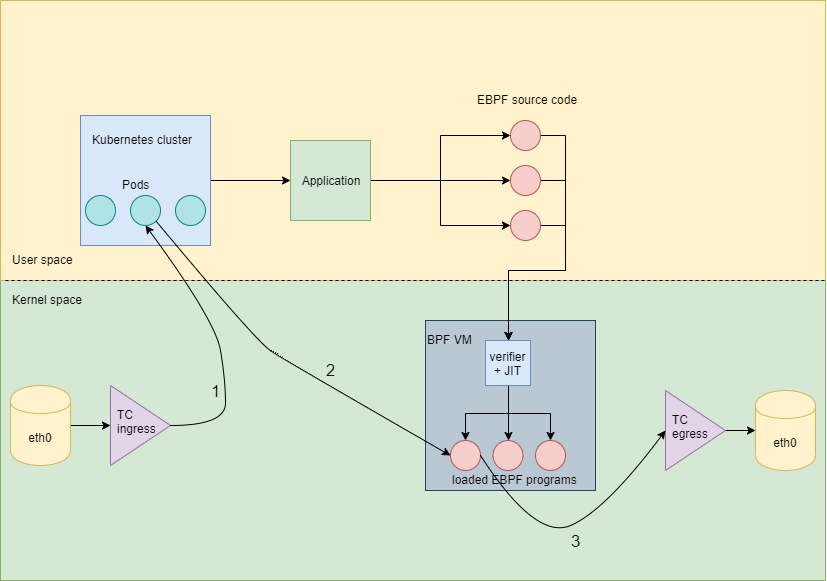
\includegraphics[width=\textwidth]{images/architecture.png}
	\caption{Application architecture}
	\label{fig:app-arch-2}
\end{figure}
\noindent
The proposed solution consists of three main parts.
\begin{enumerate}
	\item The Kubernetes cluster: in most cases, this is a preexisting system, unless specifically set up for testing the application
	\item The application: continuously monitors the state of the Kubernetes cluster and applies limits based on its configuration
	\item The eBPF Virtual Machine: loads the eBPF programs, verifies their code and runs them whenever a packet arrives on the target ingress / egress interface.
\end{enumerate}

These main parts and technologies, with the addition of some glue, play together to form a versatile yet extensible ecosystem and solve the proposed problem.

\newpage
\section{Underlying technologies}
\subsection{Kubernetes}
Kubernetes, or K8S for short, is an open source container orchestration system that is simply too vast to properly explain in a BSc thesis. It supports automatic deployment and scaling of containerized workloads and services. It also works as a base for an ecosystem that is built around it. The project was open-sourced by Google~\cite{google} in 2014 and gained prominence in the last few years. Today, it is a mature platform to depend on - no matter what kind of service one is running. Chances are, if scale is a concern, Kubernetes is the answer.

\subsubsection{Why use Kubernetes?}
Today, users of online services are used to a high standard - fast response times, no downtime, no data loss, easy usage. This standard requires modern solutions; a single machine in one's garage running a LAMP~\cite{lamp} (Linux, Apache, MySQL, PHP) stack will not cut it anymore. In fact, oftentimes a garage full of server equipment will not cut it.

Scaling this big is hard, though, and This is what Kubernetes is trying to mitigate. Using containers, software becomes more manageable. Containers provide an unified system services can run on, without having to care about what kind of system they run on. These can then be started on-demand, for example when there is a load spike, or another container dies. This ensures that the available workforce is always present and can endure the load, no matter what size it is.

\noindent
The main benefits of Kubernetes are:
\begin{itemize}
	\item Load balancing: Kubernetes can ensure that no host gets overloaded and the services remain stable
	\item Scalability: Containers can be started and stopped on-demand. The deployments always fit to the load.
	\item Automation: Kubernetes automatically modifies its state at a given rate to meet the requirements set by the sysadmins.
	\item Self-healing: Dead or non-responding pods are automatically restarted.
\end{itemize}

\subsubsection{Kubernetes architecture}
\begin{figure}[H]
	\centering
	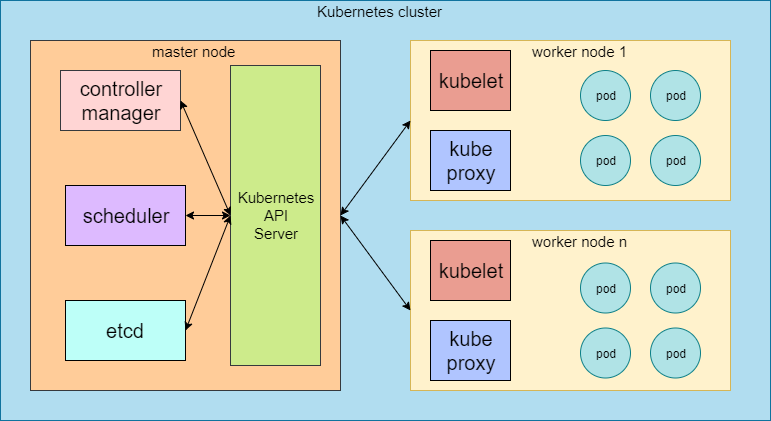
\includegraphics[width=\textwidth]{images/kube-arch-1.png}
	\caption{Basic architecture of Kubernetes internals}
	\label{fig:kube-arch}
\end{figure}
A Kubernetes cluster is made up from two primary components: the control plane (also called the master node), and one or more worker nodes. The former contains the logic required to orchestrate the latter.

\subsubsection{Master node}
The master node has a single instance and combines multiple already existing - and proven by time - technologies that make Kubernetes so flexible.

The core of everything is the kube-apiserver. It provides an \underline{\gls{api}} to configure and monitor everything while also communicating with other parts of the cluster, such as etcd~\cite{etcd}, the kube-scheduler, and controller manager. Etcd is used as a reliable key-value storage that holds every piece of data related to the cluster. The kube-scheduler is responsible for assigning worker nodes to Pods that need to be started. Finally, the controller-manager changes the state of the cluster to always fit the load best.

The master node can run on any machine in a cluster, but typically it is either on the same machine as the worker nodes (in \underline{\gls{on-premises}} cases), or it is hosted by a cloud provider.

\subsubsection{Worker node}
The worker nodes - their number can vary - are the workhorse of the cluster. They are used to run Pods that run the target applications - be they online services or \underline{\gls{ml}} learning algorithms.

The worker nodes are controlled by a program called kubelet. Kubelet manages the Pods and the \underline{\gls{cri}}, the container runtime, which is generally, but not limited to Docker~\cite{docker} or containerd~\cite{containerd}.

Another tool called kube-proxy implements the overlay network used by Kubernetes. This is required because the communication between pods should be private; unauthorized access from the outside is unwanted. Similarly, the Pods should not access resources outside the cluster that are not explicitly configured.

\subsubsection{Concepts}
\textbf{Pods} are the smallest components used in Kubernetes. As the name suggests, they represent a group of containers that are closely related and should be handled together. Pods are fast to start and shut down by design, as they are often rotated for various reasons, examples being scaling up and down, starting new pods to replace dead ones, etc. \\

\textbf{Services} are used as an abstraction over a group of Pods. Since usually there are more than one pods, something has to act as a \underline{\gls{load-balancer}} to distribute the requests between the running pods. They are also used to expose an application to the (inner) network. \\

\textbf{Ingresses} act as a reverse-proxy and provide an unified channel external requests can enter through. Depending on the specific implementation (for example, NGINX~\cite{nginx} and Traefik~\cite{traefik} are solid ones, this thesis project uses the latter), they provide various features, the most important ones being dns/port based routing to services, load balancing and \underline{\gls{ssl}} termination. \\

These aforementioned, rather simple concepts enable the sysadmins to build complex, yet highly performant clusters that scale well under even the most extreme loads.

\begin{figure}[H]
	\centering
	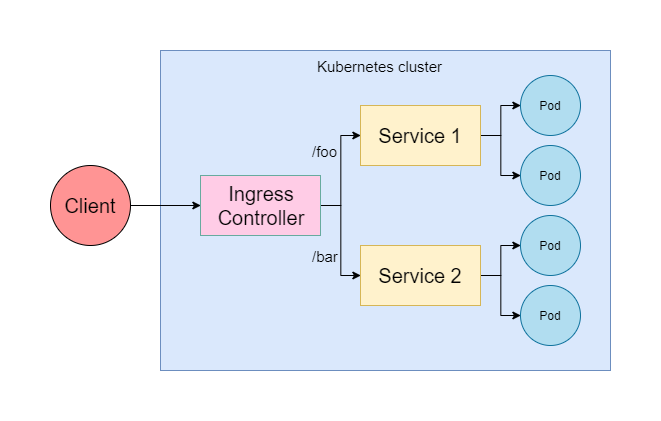
\includegraphics[width=\textwidth]{images/kube-arch2.png}
	\caption{A simple Kubernetes cluster configured with two microservices}
	\label{fig:kube-cluster}
\end{figure}

In the figure above, an ingress controller is used to let in traffic on the HTTP and HTTPS ports, routing them to two services that abstract the pods - 2 each - running web microservices. This simple example shows how the Kubernetes objects interact and enable operators to build bloat-less systems.

\newpage
\subsection{eBPF}
eBPF~\cite{ebpf} emerged from BPF~\cite{bpf-original}, which is a complex system that leverages a virtual machine with a limited instruction set to run user-made programs in the kernel space. This avoids the need to copy each network packet to the user space, granting significant speed gains. These BPF programs interact directly with raw network sockets. \\

Before loading the programs into the kernel, BPF analyzes the source files to make sure they contain only permitted instructions. The instructions in these files are then run sequentally. The execution of the programs is event-driven; they can be attached to various events, such as the arrival or transmission of a network packet.
 
\subsubsection{BPF VM}
BPF uses a virtual machine that runs code made up from a set of instructions conforming to the format described in Code~\ref{bpfinsn}.
\lstset{caption={BPF instruction format}, label=bpfinsn}
\begin{lstlisting}[language={C++}]
struct bpf_insn {
	__u16	code; // Opcode
	__u8	jt;	  // Jump if true
	__u8	jf;   // Jump if false
	__u32	k;    // Instruction-dependent field
};
\end{lstlisting}

The programs are made up from these instructions and are represented as an array of 4-\underline{\gls{tuple}}, run in a sequence.

\lstset{caption={BPF program format}, label=bpfprog}
\begin{lstlisting}[language={C++}]
struct bpf_program {
	unsigned short len; // Number of instructions
	struct sock_filter __user *filter;
};
\end{lstlisting}

The BPF virtual machine has a rather simple architecture. A 32 bit wide register - called A - is used as an accumulator and another one - called X - is used as a helper register. The VM also has a 32 bit wide "scratch memory store" - called M - that can store up to 16 values.

BPF has a simple \underline{\gls{risc}} (Reduced Instruction Set Computing) instruction set consisting of load, save, jump, arithmetic and logic operations. A program of these instructions is usually denoted as an array of 4-tuples. \\
 
Full list of instructions:
\begin{center}
 \begin{tabular}{||c c c||} 
 \hline
 Instruction & Addressing mode & Description \\ [0.5ex] 
 \hline\hline
  ld & 1, 2, 3, 4, 12 & Load word into A \\
  \hline
  ldi &  4 & Load word into A \\
  \hline
  ldh &  1, 2 & Load half-word into A \\
  \hline
  ldb & 1, 2 & Load byte into A \\
  \hline
  ldx & 3, 4, 5, 12 & Load word into X \\
  \hline
  ldxi & 4 & Load word into X \\
  \hline
  ldxb & 5 & Load byte into X \\
  \hline
  \hline
  st & 3 & Store A into M[] \\
  \hline
  stx & 3 & Store X into M[] \\
  \hline
  \hline
  jmp & 6 & Jump to label \\
  \hline
  ja & 6 & Jump to label \\
  \hline
  jeq & 7, 8, 9, 10 & Jump on A == <x> \\
  \hline
  jneq & 9, 10 & Jump on A != <x> \\
  \hline
  jne & 9, 10 & Jump on A != <x> \\
  \hline
  jlt & 9, 10 & Jump on A <  <x> \\
  \hline
  jle & 9, 10 & Jump on A <= <x> \\
  \hline
  jgt & 7, 8, 9, 10 & Jump on A >  <x> \\
  \hline
  jge & 7, 8, 9, 10 & Jump on A >= <x> \\
  \hline
  jset & 7, 8, 9, 10 & Jump on A \&  <x> \\
  \hline
\end{tabular}
\captionof{table}{BPF instructions part 1}
\end{center}

\newpage
\noindent
Continued:
\begin{center}
 \begin{tabular}{||c c c||} 
 \hline
 Instruction & Addressing mode & Description \\ [0.5ex] 
 \hline\hline
  add & 0, 4 & A + <x> \\
  \hline
  sub & 0, 4 & A - <x> \\
  \hline
  mul & 0, 4 & A * <x> \\
  \hline
  div & 0, 4 & A / <x> \\
  \hline
  mod & 0, 4 & A \% <x> \\
  \hline
  neg & & !A \\
  \hline
  and & 0, 4 & A \& <x> \\
  \hline
  or & 0, 4 & A | <x> \\
  \hline
  xor & 0, 4 & A \^ <x> \\
  \hline
  lsh &  0, 4 & A << <x> \\
  \hline
  rsh & 0, 4 & A >> <x> \\
  \hline
  tax & & Copy A into X \\
  \hline
  txa & & Copy X into A \\
  \hline
  \hline
  ret & 4, 11 & Return \\
  \hline
\end{tabular}
\captionof{table}{BPF instructions part 2}
\end{center}

\newpage
There are multiple addressing modes each having its own quirks. The table below explains their behavior.
\begin{center}
 \begin{tabular}{||c c c||} 
 \hline
   Addressing mode & Syntax & Description  \\ [0.5ex] 
 \hline\hline
   0 & x/\%x & Register X \\
   \hline
   1 & [k] & BHW at byte offset k in the packet \\
   \hline
   2 & [x + k] & BHW at the offset X + k in the packet \\
   \hline
   3 & M[k] & Word at offset k in M[] \\
   \hline
   4 & \#k & Literal value stored in k \\
   \hline
   5 & 4*([k]\&0xf) & Lower nibble * 4 at byte offset k in the packet \\
   \hline
   6 & L & Jump label L \\
   \hline
   7 & \#k,Lt,Lf & Jump to Lt if true, otherwise jump to Lf \\
   \hline
   8 & x/\%x,Lt,Lf & Jump to Lt if true, otherwise jump to Lf \\
   \hline
   9 & \#k,Lt & Jump to Lt if predicate is true \\
   \hline
  10 & x/\%x,Lt & Jump to Lt if predicate is true \\
   \hline
  11 & a/\%a & Accumulator A \\
   \hline
  12 & extension & BPF extension \\
   \hline
\end{tabular}
\captionof{table}{Addressing modes of instructions}
\end{center}

\newpage
\subsubsection{eBPF}
\label{sec:ebpfrules}
BPF was originally proposed in 1992, having seen low to moderate success. eBPF, which builds on the original BPF implementation, first appeared in Linux kernel 3.18~\cite{kernel-318} released in 2014 and became widely adopted in the last few years. However, it is still somewhat of an underground technology, as it requires more-than-average knowledge about the Linux kernel and its use cases are quite narrow.

The relative bigger success of eBPF is mainly due to the fact that it not just extended, but reworked the technology from ground up. The VM was expanded to support 64 bit architectures and a variety of things absent form the predecessor.

\subsubsection{eBPF VM}
The re-implemented eBPF VM architecture has eleven general-purpose 64 bit wide registers (r0 - r10) that can also be used in 32 bit mode. R10 is \underline{\gls{read-only}} and contains the \underline{\gls{fp}} It also has a \underline{\gls{pc}} and a 512 byte long \underline{\gls{stack}}.

This new architecture also brought a new instruction format along described in Code~\ref{ebpfinsn}.
\lstset{caption={eBPF instruction format}, label=ebpfinsn}
\begin{lstlisting}[language={C++}]
struct ebpf_insn {
	__u8	code;		// Opcode 
	__u8	dst_reg:4;	// Destination register
	__u8	src_reg:4;	// Source register
	__s16	off;		// Signed offset
	__s32	imm;		// Signed immediate constant
};
\end{lstlisting}

The new instruction format made it necessary to update the instructions themselves as well. The base stayed the same, but it was extended to support 64 bit wide data and added several new features, for example, function calls and proper branching instructions. The list is too long to include, however it is freely available~\cite{ebpf-instructions}.

This new architecture is much more powerful than the limited functionality the original BPF system provided. This introduced the requirement of having a \underline{\gls{verifier}} that scans the code and rejects to load anything outside the allowed parameters. eBPF has three main rules that make it safe to use.
\begin{itemize}
	\item Only forward jumps are allowed. This ultimately means that loops are forbidden, guaranteeing the termination of the program.\footnote{Since Kernel 5.3, bounded loops are allowed. See https://lwn.net/Articles/794934/.}
	\item All memory accesses are validated. The kernel must not allow the programs to tamper around in the memory.
	\item The program must have no more than 4096 instructions.\footnote{Since Kernel 5.2, the limit was pushed out to one million. See https://www.spinics.net/lists/netdev/msg561449.html.}
\end{itemize}

These basic rules together ensure that all BPF programs run fast and terminate without exceptions.


\subsubsection{eBPF for packet filtering}
Even though BPF's original purpose was - as the name suggests - packet filtering, eBPF broadened the tool's functionality. Nowadays, a hook can be virtually added anywhere on the machine, be it in the kernel or user space code. These can be done using \underline{\gls{kprobe}}s and \underline{\gls{uprobe}}s respectively.

Staying on the topic, packet filtering can be done through attaching eBPF programs to ingress or egress \underline{\gls{socket-buffer}}s. Ingress socket buffers are where transmitted data is passed to a process, and egress socket buffers are where the process outputs data that gets transmitted back onto the network. These socket buffers are located in kernel space and are managed by the Linux \underline{\gls{tc}}. \\

An example of a simple bandwidth limiter eBPF program would be attached to the egress of a process. It would either let packets pass, or throw them away based on their length and the time elapsed since the last packet. More sophisticated solutions would delay the packets and not throw them away. This latter is called \underline{\gls{edt}} filtering.

\newpage
\subsection{Go}
Golang~\cite{go} is an open-source programming language that focuses on code simplicity, efficiency and reliability. It has a very opinionated view on how code should look and behave, which is referred to as idiomatic way. Go also has a wide set of concurrency mechanisms which make it perfect for writing networking and multi-core applications. \\

The language was designed at Google~\cite{google} by Rob Pike~\cite{rpike}, and Ken Thompson~\cite{kthompson} themselves, among others, first released in 2012~\cite{go-1}.

Under the hood, Go is a \underline{\gls{compiled}} and \underline{\gls{statically-typed}} language that resembles C~\cite{c}, but unlike this latter, it has a \underline{\gls{garbage-collector}}, it is \underline{\gls{memory-safe}}, and has an actually usable standard library. \\

The project uses Go as the main language for the application because there were no special requirements, any other general-purpose languages would have worked, for example C++ or Python. Go's preference of simplicity and my familiarity with the language were the main reasons to pick it. \\

One important thing about Go is that it does not support most classic \underline{\gls{oop}} paradigms such as inheritance or polymorphism. Instead, Go has an unique take on what OOP should be like. This by the way, often throws off developers getting acquainted with the language as it feels alien at first. For this same reason, the thesis does not include any complex OOP features - they would be pointless anyway as the internal structure is kept simple.

\newpage
\subsection{Other Linux technologies}
\subsubsection{Control Group V2}
Another relatively recent technology utilized by the thesis project is cgroup v2~\cite{cgroup}. Cgroup is a hierarchical system where groups can contain other groups and every process belongs to exactly one group. These groups are addressable and are used to distribute system resources, for example \underline{\gls{cpu}} capacity or usable \underline{\gls{ram}}. \\

The old V1 version is now deprecated and is superseded by V2. It unifies the then scattered layout of the hierarchy in one \underline{\gls{tree}}. Though it is widely available, some projects still do not fully support it, one example being K3S (a K8S distribution, also used by this project) until very recently.

The thesis project uses the cgroup V2 system to address processes during the eBPF attachment procedure.

\subsubsection{Tools}
\textbf{Bpftool}~\cite{bpftool} is a Linux utility that is used to load and unload BPF code as well as to inspect BPF logs and maps. This latter can be done by running the following command.
\begin{verbatim}
$ sudo bpftool p t
\end{verbatim}

\textbf{Clang}~\cite{clang}, part of the LLVM project is a C/C++ compiler that is able to compile eBPF bytecode. At the time of writing this thesis, this compiler is the most reliable way to generate eBPF programs.

\newpage
\section{Implementation}
\subsection{The application}
This section will explain the actual implementation of the application and its subprograms. The application is written in Go because of its simplicity and robustness. As the main application is just orchestrating other technologies to work together, no complex structure was required.

\begin{figure}[H]
	\centering
	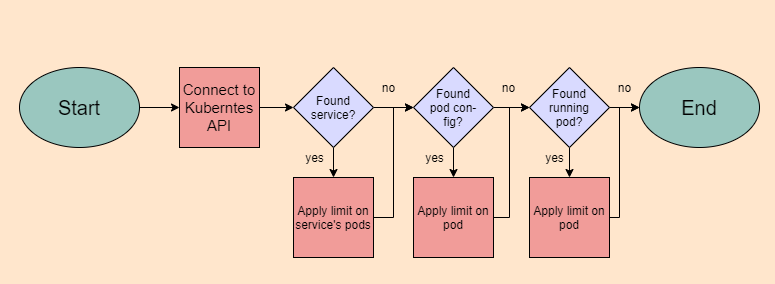
\includegraphics[width=\textwidth]{images/loading.png}
	\caption{Application logic flow}
	\label{fig:app-flow}
\end{figure}

The structure of application follows a simple workflow. On startup, the application connects to the Kubernetes API, sweeping the cluster for services and pods that require eBPF programs to get hooked on. It also starts to watch events happening in the cluster, in case pods get replaced.

When finding a service that is configured to use a limit, the corresponding pods are also searched and the limit is applied on them. When finding a direct pod limit, it is directly applied.

The process of applying eBPF programs that implement limits consists of compiling the eBPF programs with the given parameters, loading them into the kernel, and attaching these programs to the cgroup of the given pod's processes.

\subsubsection{Startup}
In Go programs, the entry point is a \texttt{main()} function in the package main. This is where the program flow starts.

When starting the application, the first thing that happens is locating the kubeconfig file. This file can be either in the home folder of the user, or anywhere else - this location can be passed to the application through a command-line parameter. After locating the kubeconfig file, the contents are interpreted and the application attempts to connect to the Kubernetes API. \\

A struct - the Go equivalent of class - called PodManager is responsible for the business logic. 
\begin{figure}[H]
	\centering
	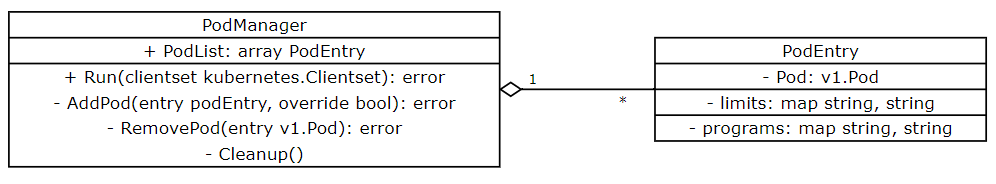
\includegraphics[width=\textwidth]{images/uml.png}
	\caption{Class diagram of the pod manager code section}
	\label{fig:uml}
\end{figure}

The PodManager holds all the data related to the program execution - information about pods and their corresponding limits and eBPF programs - and also contains the core logic. The execution start when the \texttt{Run()} method is called. This method executes the following 3 steps in a strict order:

\begin{enumerate}
	\item Looking for configured services: most often, limits will be applied on this level.
	\item Looking for configured pods and deployments: this must come after looking for services; pod-level limits overwrite service-level ones, providing a hierarchical solution.
	\item Setting up an even watcher for pods through the Kubernetes API: this step comes last because at this point, we only want to find changes in the cluster.
\end{enumerate}

When looking for services and pods, the software is checking their annotation parameter to see if there are any limits present. In the last step, the event watcher is set up and it runs until the application exits. This enables dynamic loading and unloading of eBPF programs whenever the cluster is changed.

\subsubsection{eBPF program loading}
The first step of eBPF program loading is to actually compile the object code. This is done using the Clang compiler. The pre-implemented programs' sources are stored in the \texttt{bpf} folder. Every program is compiled independently to provide custom settings through the macros.

During compilation, the kernel headers are linked to the object code, and specific macros are set depending on which program is being compiled. These macros are used to bypass a limitation of the eBPF VM, namely that it does not allow the programs to be parametrized. Although eBPF does support maps that are accessible from user space, these do not fit the use case. \\

After compilation, the next step is to actually load the object-code into the kernel. This is done through a system call, which is done by the bpftool utility automatically invoked though command line. Upon loading the object-code, the eBPF verifier examines the code and makes sure it is safe to run. If the verifier accepts the code, it gets compiled to machine code. The internal compiler also optimizes the code, making it run at speeds similar to natively compiled kernel code. \\

Once the eBPF program is loaded into the kernel, it must be attached to a process. This process is referred to by its cgroup, which is found in the \texttt{/sys/fs/cgroup/} folder. After the attachment, the system is live and the limits should instantly begin to take effect. This can be made sure using the following command.
\begin{verbatim}
$ sudo bpftool p t
\end{verbatim}

If the process finished successfully, the command should show packet transmission and whether they were dropped or not.

\subsubsection{Cleanup}
On exiting (and pod removal in the cluster), cleanup is done. This includes removing temporary artifacts as well as unloading and deattaching eBPF programs - even though they automatically get cleaned up if the process they are attached to stop. This process is done for the sake of completeness.

These processes happen in reverse order - meaning first the program is deattached from the cgroups, after which they are unloaded, and finally, the artifacts (the object files) are deleted.

\newpage
\subsection{Implemented rules}
Although the thesis project is extensible with custom user-made eBPF programs, it comes with prebuilt ones that cover the most frequently required features. The following sections describe the inner working of these programs.

\subsubsection{Bandwidth limit}
The bandwidth manager's sole purpose is to limit the bandwidth used by a specific Pod's \underline{\gls{ingress}} or \underline{\gls{egress}}. To reach this goal, it employs an algorithm called \underline{\gls{tbf}} which drops packets that are too big compared to the time elapsed since the last one. This is a rather simple solution, keeping the average bandwidth below a specified threshold. \\

The pros of TBF include simplicity and high processing speed. This can be useful in cases where low \underline{\gls{latency}} is an absolute necessity, for example serving multimedia content on the web. The high speed of the algorithm is due to its simplicity; the low latency is guaranteed by the fact that packets are either instantly let-through, or dropped. Below-limit bandwidth is always instantly forwarded. \\

The cons arise from the nature of the algorithm - packets above the bandwidth limit get dropped. This means that only \underline{\gls{tcp}} transmissions are reliable, as they resend packets that were not acknowledged. \underline{\gls{udp}} does not do this, requiring proper user-made \underline{\gls{netcode}} to handle dropped packets. \\

Staying at the topic of \underline{\gls{transport-layer}} protocols, TCP also shapes the speed of the data transmission dynamically. This is helpful because as packets get dropped, TCP throttles the speed, requiring the bandwidth manager to drop less packets. UDP does not have any similar features.

\newpage
\textbf{The TBF algorithm} uses a bucket that gets filled with "tokens". Packets take tokens to send, and if a packet would  completely drain the bucket, it gets dropped, otherwise let through. More formally:
\texttt{
\begin{enumerate}
	\item Tokens are added to a bucket with 1/ rate interval.
	\item A bucket can hold at most b tokens.
	\item When a packet arrives (of length p):
	\begin{enumerate}
    	\item If the bucket has more than p tokens, the same amount is removed and the packet is let through.
    	\item Otherwise, the packet is discarded.
    \end{enumerate}
\end{enumerate}
}
eBPF is event-driven - in this case, these events are packet arrivals on either the ingress or the egress interface - therefore this algorithm requires slight modifications to work properly, namely the token addition is the part that requires discrete time steps instead of being continuous. The implemented algorithm is the following.
\texttt{
\begin{enumerate}
	\item When a packet arrives:
	\item Calculate the time between the last packet and the current packet's arrival as dT.
	\item Add dT * rate amount of tokens to the bucket
	\item If the bucket has more than p tokens, the same amount is removed and the packet is let through.
	\item Otherwise, the packet is discarded.
	\item Update the time of the last packet's arrival
\end{enumerate}
}
The algorithms may slightly differ, but in essence, both implement the same idea: only let through packets through where the average bandwidth calculated as \texttt{packet size * (time of last packet - time of current packet)} is below the threshold. This limits the maximal available bandwidth.

There are also other TBF algorithms that extend the basic idea of it, though they are not implemented in the project as they are not required for the original purpose. Examples include the leaky bucket and the hierarchical token bucket algorithms.

\subsubsection{Packet loss}
Simulating packet loss is useful in cases where network-congestion testing is important. It can be configured for Pods' ingress or egress interfaces. There are two variations provided by the implementation, one using uniform and the other using exponential distribution.

Simulating probability-based things is very difficult without \underline{\gls{float}} or an usable standard library. Unfortunately, neither of those are available in the Linux kernel. To further complicate things, a \underline{\gls{rng}} is also required, not provided by the kernel by default. \\

For random-numbers, both implementations use the function \texttt{bpf\_get\_prandum\_u32()}. This generates a random 32 bit value which is then used as a base for both distributions. The absence of floating-point numbers is circumvented by only using integer calculations; this does lose precision but for the use case, it is good enough. \\

Using the \textbf{uniform-distribution}, a percentage of packets can be dropped. This comes useful simulating congestion that happens on a regular basis, such as crowded Wi-Fi. This version of the loss manager is pretty straightforward, requiring little explanation. The random 32 bit number is interpreted as an unsigned integer modulo 100, and the output is compared to the given percentage provided in configuration. The packet is then passed through or dropped based on this. \\

The \textbf{exponential-distribution} has a threshold above which it throws packets. Using this distribution, edge-cases can be simulated - as the top-end of the distribution is rather rare.

Exponential distribution can be calculated from uniform one. Given a variable U conforming to uniform-distribution between [0,1), the following formula can be used to calculate the exponential-distributed value:
$$\xi = -\frac{1}{\lambda}\ln(1-U)$$

\newpage
The implementation is somewhat awkward because of the absence of floating point integers and math libraries, this equation can not be used. Instead, since no better tools are available inside the kernel, a lookup table containing a predefined exponential curve is used. This is somewhat of a hack-ish solution, but after careful consideration, it was chosen not only because of the lack of better methods, but also for its speed. Very few - if any - other solutions beat the speed of lookup tables.

\begin{figure}[H]
	\centering
	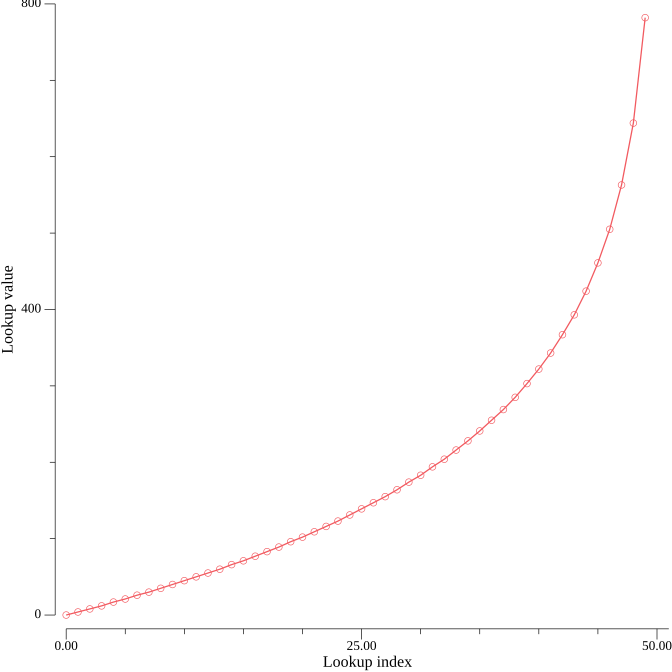
\includegraphics[width=\textwidth]{images/lookuptable.png}
	\caption{Lookup table for exponential distribution}
	\label{fig:exp-lookup-table}
\end{figure}

The lookup table itself is implemented with a switch statement, instead of using an array. This is due to the eBPF verifier, which will not let the program offset an array with a random value - not even in a sanitized and bound-checked way.

The exponential distribution code is straightforward as well. Given the random 32 bit unsigned integer modulo 50 (this number was chosen for keeping the size of the lookup table manageable), the corresponding exponential value can be found. This is then compared to a threshold, and the packet is passed through or dropped based on the comparison.


\subsubsection{EDT}
Another way of bandwidth limiting is the EDT algorithm. Instead of dropping, this algorithm delays packets to ensure the fixed bandwidth threshold is not exceeded. Due to its nature, this algorithm only works for egress interfaces, and it is not fit for our use case.

Nevertheless, it is implemented as it may come useful later in the future. It can be found in the \texttt{bpf/edt.c} file. \\

The algorithm uses a variable called \texttt{t\_next} that is set in the previous packet transmission. This variable is used to determine the earliest point the next packet can leave. The delay of a packet is calculated as \texttt{packet\_size * bitrate}. If the packet is sent after \texttt{t\_next}, it is passed through and \texttt{t\_next} is set to the current time plus the delay.

If the packet is before \texttt{t\_next}, the delay is added to the packet's timestamp and it is passed through - meaning it will be resent at a later date.

\newpage
\section{Testing}
The correctness of the software bundle is ensured with both tests and benchmarks. The tests are performed on the code, while benchmarks are measured on the running systems.

\subsection{Unit tests}
Since the main application is kept simple, meaning it has neither complex structure or user-interface, testing the code base is simple as well, as there are only a few things that can be tested. \\

Due to how Go implements the type system, \underline{\gls{mock}}ing is rather verbose. Polymorphism is achieved through interfaces, which are types having only methods. Actual types can implement these, and therefore the interface itself, and can be passed as such. This means mocking for example the Kubernetes API would mean all of its functions need to be re-implemented, which is simply not feasible. For this reason, dependencies such as the Kubernetes API are not tested; they should be tested in a stand-alone manner anyway. \\

\noindent
The following basic features are tested:
\begin{itemize}
	\item Compiling programs
	\item Deleting programs
	\item Loading programs
	\item Unloading programs
\end{itemize}

The eBPF programs themselves cant be tested in any way due to their specific format and the fact that tests can not be run in the Linux kernel.

\newpage
\subsection{Benchmarks}

The benchmarks are run on both pre-written managers to ensure proper functionality. 

\subsubsection{Bandwidth manager}
The bandwidth manager limits the maximum usable bandwidth for a given pod, therefore the sustained bandwidth is measured to ensure these metrics remain below threshold. For measurement, iperf3~\cite{iperf} was used in TCP mode, the tests were run for one minute for each limit. The bandwidth limiter was attached to the egress interface of the sending process.

The findings can be found in Figure~\ref{fig:bandwidthbench1}. As it can be seen, the bandwidth conformed to the limits pretty closely, with errors here and there. The maximum measured error was 4.7\%, which occurred in the 600 Mbps run.

\begin{figure}[H]
	\centering
	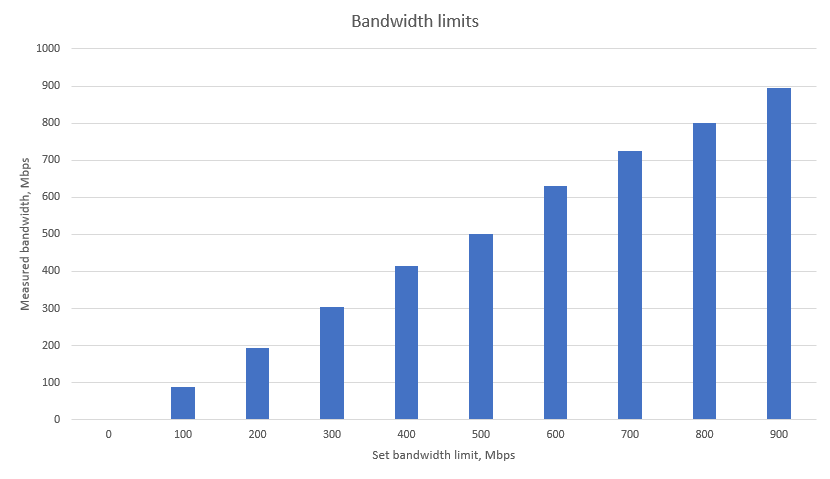
\includegraphics[width=\textwidth]{images/bandwidth.png}
	\caption{Bandwidth benchmarks}
	\label{fig:bandwidthbench1}
\end{figure}

\subsubsection{Loss manager}
The loss manager has two different mechanisms to calculate packet drop chances. The common thing between these two is that both are using random numbers in a way or another to decide which packet to drop. Both are measured using a small utility that tries to send 100.000 UDP (this is important because TCP will try to re-send non-acknowledged packets) packets. Similarly to the bandwidth manager, the eBPF programs are attached to the egress interface to the sending process. \\

The first version of loss manager is using uniform distribution to drop a percentage of packets. The accuracy of the method can be seen in Figure~\ref{fig:lossbench1}. Since there is no time or packet size data in play here, and the random generator is reasonable reliable, the measured packets follow the targets very well.

\begin{figure}[H]
	\centering
	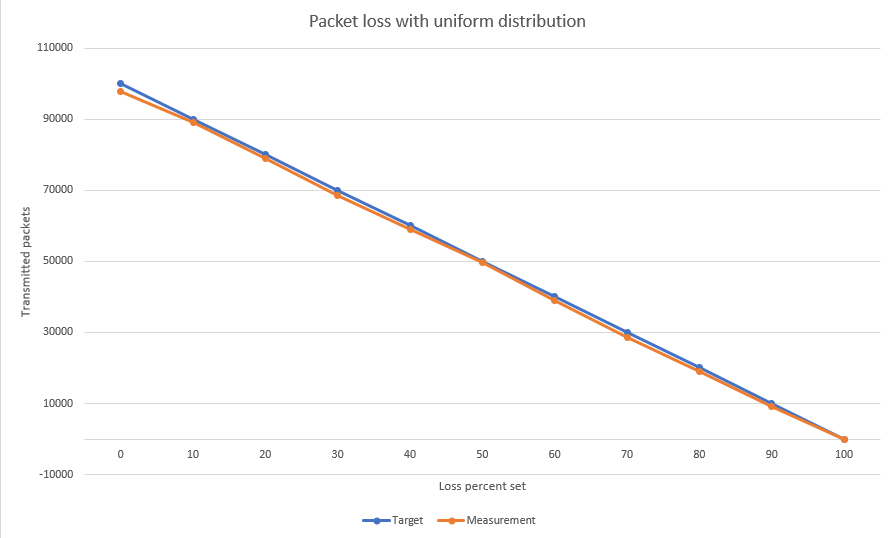
\includegraphics[width=\textwidth]{images/loss1.png}
	\caption{Loss benchmarks with uniform distribution}
	\label{fig:lossbench1}
\end{figure}

The second version uses exponential distribution - enabling the users to simulate events that occur in edge cases. The measurements can be seen in Figure~\ref{fig:lossbench2}. There is a slight deviation from the target in the middle of the plot, this is due to the usage of lookup tables instead of a continuous function - a little precision is sacrificed for speed. However, the measurements are still relatively close to the target values, making the exponential distributed packet loss an usable feature.

\begin{figure}[H]
	\centering
	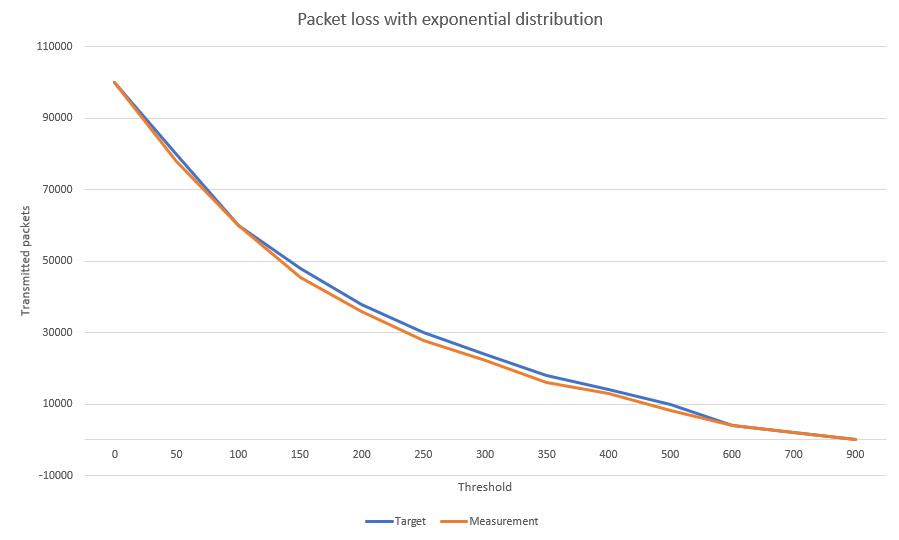
\includegraphics[width=\textwidth]{images/loss2.png}
	\caption{Loss benchmarks with exponential distribution}
	\label{fig:lossbench2}
\end{figure}


\chapter{Summary}

The implemented application simulates various conditions on service or pod level by applying eBPF filters on the pods' ingress or egress socket buffers. This is done through the Kubernetes API. \\

Based on the benchmarks, the implementation is conforming to the proposed specifications, requiring no further fine-tuning. The application does its job - simulating various network conditions - and it is also extensible, having potential for more complex filters. \\

The application can be extended in various ways in the future. Two main possibilities are a graphical user interface and adding robustness (more portability, not requiring root privileges).
\cleardoublepage

\chapter{Summary} % Conclusion
\label{ch:sum}

Lorem ipsum dolor sit amet, consectetur adipiscing elit. In eu egestas mauris. Quisque nisl elit, varius in erat eu, dictum commodo lorem. Sed commodo libero et sem laoreet consectetur. Fusce ligula arcu, vestibulum et sodales vel, venenatis at velit. Aliquam erat volutpat. Proin condimentum accumsan velit id hendrerit. Cras egestas arcu quis felis placerat, ut sodales velit malesuada. Maecenas et turpis eu turpis placerat euismod. Maecenas a urna viverra, scelerisque nibh ut, malesuada ex.

Aliquam suscipit dignissim tempor. Praesent tortor libero, feugiat et tellus porttitor, malesuada eleifend felis. Orci varius natoque penatibus et magnis dis parturient montes, nascetur ridiculus mus. Nullam eleifend imperdiet lorem, sit amet imperdiet metus pellentesque vitae. Donec nec ligula urna. Aliquam bibendum tempor diam, sed lacinia eros dapibus id. Donec sed vehicula turpis. Aliquam hendrerit sed nulla vitae convallis. Etiam libero quam, pharetra ac est nec, sodales placerat augue. Praesent eu consequat purus.

\cleardoublepage

\addcontentsline{toc}{chapter}{Glossary}
\printglossaries
\cleardoublepage


% Ábrajegyzék (opcionális) - 3-5 ábra fölött érdemes
% List of figures (optional) - useful over 3-5 figures
\addcontentsline{toc}{chapter}{\lstfigurelabel}
\listoffigures
\cleardoublepage

% Bibliography (mandatory)
\addcontentsline{toc}{chapter}{\biblabel}
\printbibliography[title=\biblabel]

\end{document}